\section{Analysis: Privileged Context Reduces Forking}
\label{sec:analysis}

Section~\ref{sec:results} isolates when privileged-context distillation damages
thinking models: the degradation appears most clearly at long rollout budgets
and grows with the density of the teacher's privileged context. We next analyze
a possible mechanism: privileged context changes the per-token distillation
signal on forking tokens, which mark uncertainty or redirection, and trained
students produce fewer such tokens at evaluation. The evidence has three
parts. First, privileged context shifts the fork--lock structure of
thinking-model rollouts
(\S\ref{sec:fork-lock-analysis}). Second, at these positions, the token-level
distillation signal reverses on self-correction and uncertainty markers
(\S\ref{sec:token-signal-analysis}). Third, trained \opsd{} students produce
fewer deliberation markers at evaluation
(\S\ref{sec:trained-student-deliberation}).

\subsection{Privileged context shifts the fork--lock distribution}
\label{sec:fork-lock-analysis}

Following the SSD diagnostic of \citet{zhang2026embarrassingly}, we distinguish
\emph{fork} positions from \emph{lock} positions. A fork is a high-entropy
position where several plausible continuations remain available and may lead to
different reasoning paths; a lock is a locally constrained position where the
continuation is comparatively determined. We classify positions from the
teacher distribution along sampled rollouts with a top-candidate dominance
heuristic: a position is a fork when the top candidate has probability below
$0.25$, and a lock when the top candidate has probability above $0.65$. We then
report per-rollout fork and lock rates.

\begin{figure}[t]
    \centering
        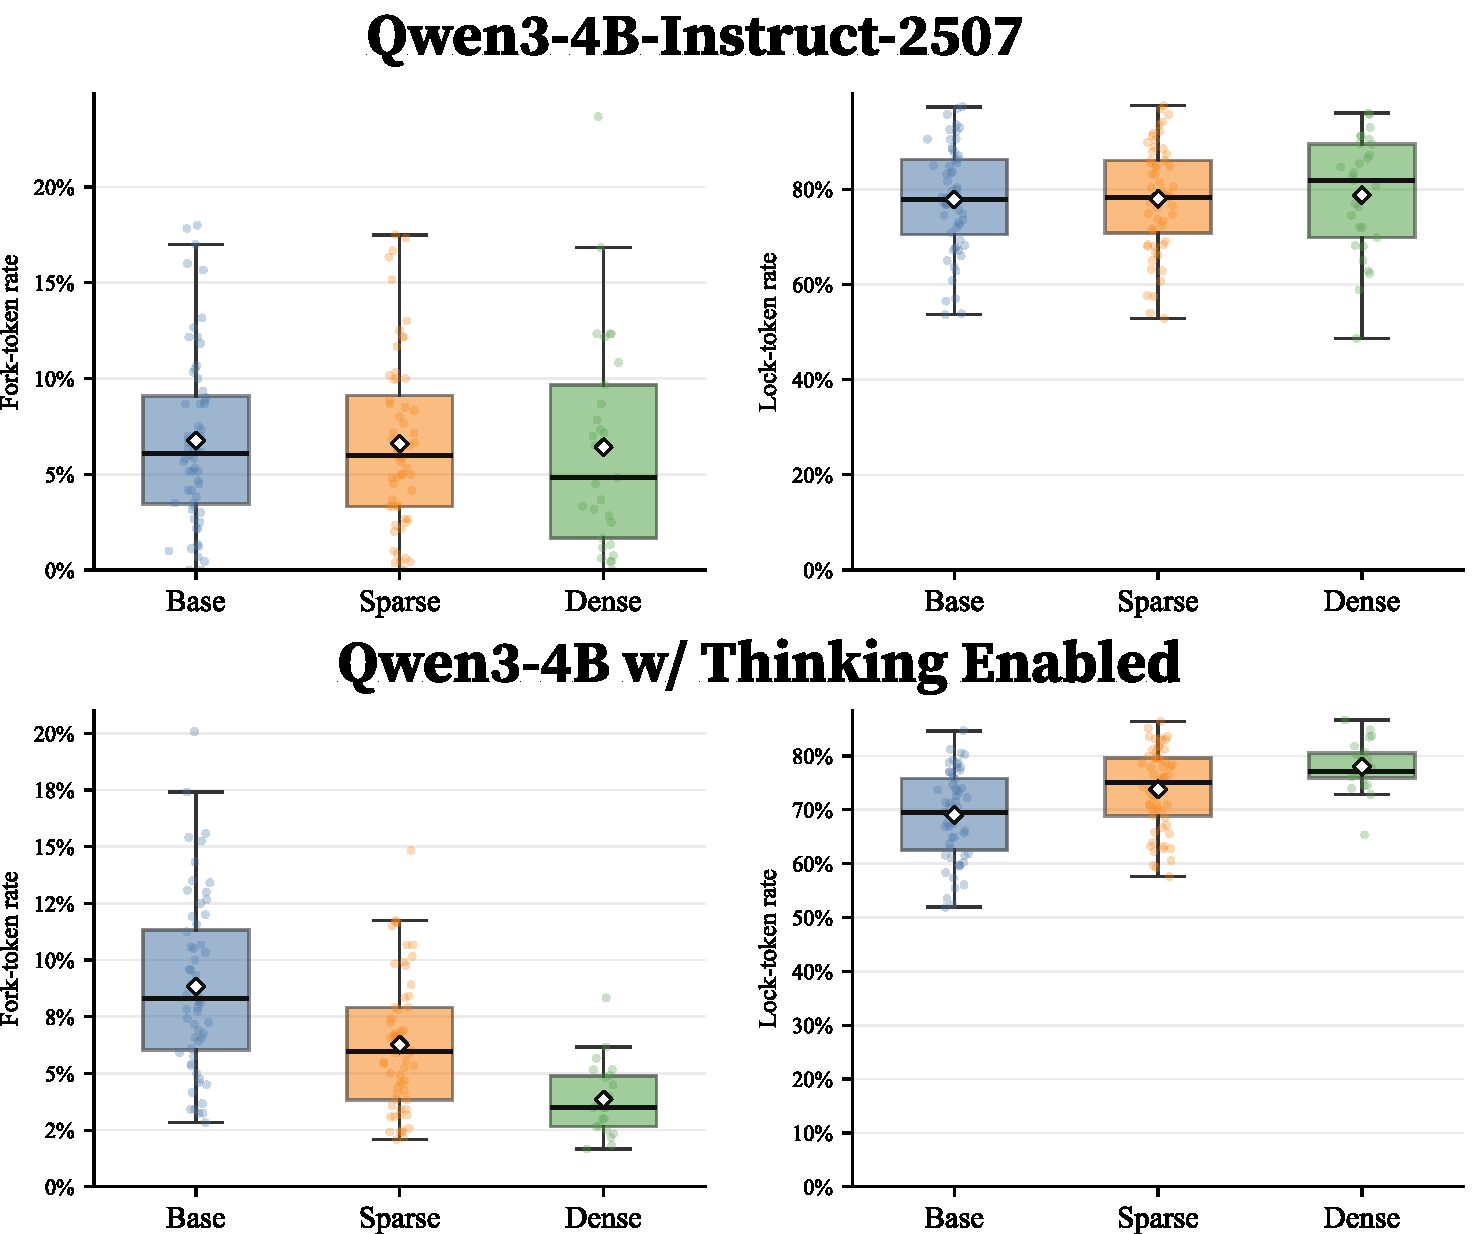
\includegraphics[width=\linewidth]{figures/qwen3-4b-qwen3-4b-instruct-2507__fork_lock_rate_boxplots.pdf}
    \caption{
    \textbf{Dense privileged context lowers fork rates in thinking rollouts but has little effect on instruction-style rollouts.}
    We compute fork and lock rates using the SSD-style diagnostic of \citet{zhang2026embarrassingly}: fork positions are high-entropy decision points with multiple plausible continuations, while lock positions are locally determined continuations. Panels show the \opsd{} side of the diagnostic for base, sparse privileged-context, and dense privileged-context conditions; the left column shows fork rate and the right column shows lock rate. For the instruction-tuned model, fork and lock rates remain mostly flat as privileged context becomes denser, with at most a small dense-context reduction in fork rate. For the thinking model, denser privileged context lowers fork rate and raises lock rate, consistent with the hypothesis that \opsd{} suppresses the branching points needed for test-time search.
    }
    \label{fig:fork_lock_context}
\end{figure}


Figure~\ref{fig:fork_lock_context} compares \qwenfourbinstruct{} and
\qwenfourb{} with thinking enabled under three teacher conditions: no
privileged context, sparse context containing the gold final answer, and dense
context containing the full gold demonstration. The two modes respond
differently. For the instruction-tuned model, fork rates remain near $0.06$ and
lock rates near $0.78$, essentially flat across conditions. For the thinking
model, denser privileged context monotonically lowers fork rates and raises
lock rates: the median fork rate drops from roughly $0.083$ to
$0.035$ between the base and dense conditions, while the median lock rate rises
from roughly $0.69$ to $0.77$.

Privileged context reshapes the rollout structure of thinking models but leaves
instruction-style rollouts essentially unchanged.

\subsection{Privileged context reverses the signal on fork markers}
\label{sec:token-signal-analysis}

The fork-rate changes in \S\ref{sec:fork-lock-analysis} align with a sign
reversal in the per-token distillation signal. Forks are often marked by short
epistemic and revision tokens such as \textit{wait}, \textit{hmm},
\textit{but}, and \textit{maybe}. These markers are lexical proxies for forking
positions, not direct measurements. We inspect the per-token teacher--student
log-ratio along sampled rollouts: positive values mean the teacher assigns more
probability than the student to the sampled token, and negative values mean the
teacher assigns less.

\begin{figure}[t]
    \centering
    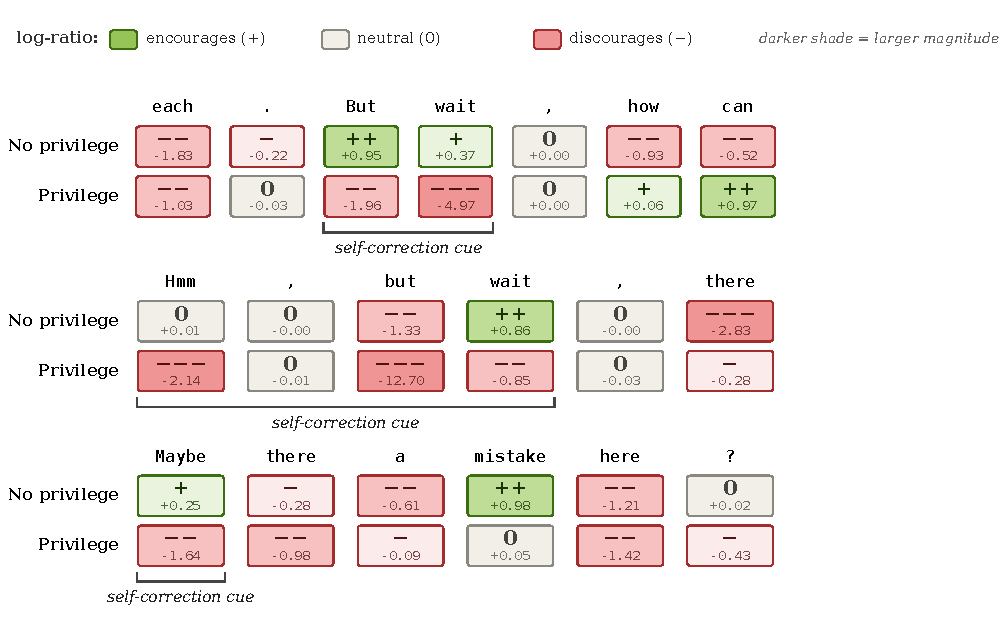
\includegraphics[width=0.95\linewidth]{figures/fig_privilege_flips_self_correction.pdf}
    \caption{\textbf{Privilege flips credit on self-correction cues, even
    when they lead to the correct answer.} Three windows from rollouts of
    a Qwen3-1.7B (Thinking) student trained against a Qwen3-8B (Thinking) teacher on
    OpenThoughts; the trajectory is identical under both teachers; only
    the teacher differs. Cells show the sign and magnitude of the
    per-token log-ratio
    $\log \pi_T(y_t \mid y_{<t}, x) - \log \pi_S(y_t \mid y_{<t}, x)$.
    \textbf{Top:} a rollout for \emph{``radius of a circle tangent to two
    concentric circles''} that ends at the wrong answer; privilege
    assigns negative advantage to \texttt{But wait} ($-1.96$, $-4.97$) and rewards the
    dismissive continuation \texttt{how can}. \textbf{Middle and bottom:}
    two windows from a rollout that reaches the \emph{correct} answer.
    Privilege still suppresses every self-correction cue, most extremely
    \texttt{but} ($-12.70$) and the hedge \texttt{Maybe} ($-1.64$). The
    pattern is consistent: the privileged teacher's positive credit moves
    away from the moments where the student notices something is off and
    onto the locally fluent continuation.}
    \label{fig:privilege-flips}
\end{figure}


Figure~\ref{fig:privilege-flips} visualizes the reversal. The trajectory is held
fixed and scored by two teachers: an unprivileged teacher that sees the same
prompt as the student, and a privileged teacher that also sees answer
information. In a rollout that ends at the wrong answer, the privileged teacher
strongly suppresses the self-correction cue \texttt{But wait} ($-1.96$,
$-4.97$) and shifts positive credit toward the locally fluent continuation
\texttt{how can}. The same pattern appears in windows from a rollout that
reaches the correct answer: the privileged teacher suppresses self-correction
cues such as \texttt{but} ($-12.70$) and \texttt{Maybe} ($-1.64$), even though
the resulting trajectory reaches the right answer.

\begin{table*}[t]
\centering
\caption{\textbf{Gold-demonstration context suppresses epistemic-token usage more than vanilla OPD.}
This token-level companion to Table~\ref{tab:qwen17_openthoughts_opsd_opd} reports marker usage by \qwenonesevenb{} on OpenThoughts. The aggregate epistemic-token density is the fraction of generated tokens in the epistemic-marker set. The remaining columns report occurrences per 1,000 generated tokens for representative revision and search markers such as \textit{wait}, \textit{recall}, \textit{check}, and \textit{hmm}. Vanilla OPD leaves the aggregate density essentially unchanged, while the gold-demonstration variant lowers both aggregate density and several named markers.}
\label{tab:qwen17_openthoughts_epistemic_tokens}
\scriptsize
\setlength{\tabcolsep}{3pt}
\renewcommand{\arraystretch}{1.12}

\begin{tabular*}{\textwidth}{@{\extracolsep{\fill}}lcccccccc@{}}
\toprule
\textbf{Method}
& \shortstack{\textbf{Epistemic token}\\[-1pt]\textbf{density}}
& \textbf{wait}
& \textbf{recall}
& \textbf{okay}
& \textbf{altern}
& \textbf{check}
& \textbf{verify}
& \textbf{hmm} \\
\midrule
\textbf{Base}
& 1.080\%
& 3.85
& 1.11
& 2.17
& 0.64
& 1.33
& 0.25
& 1.45 \\
\textbf{+OPD}
& 1.074\%
& 3.79
& 1.04
& 2.17
& 0.72
& 1.19
& 0.16
& 1.68 \\
\textbf{+OPD gold demo}
& 0.850\%
& 2.54
& 0.96
& 2.07
& 0.66
& 1.05
& 0.10
& 1.11 \\
\bottomrule
\end{tabular*}
\end{table*}


Table~\ref{tab:qwen17_openthoughts_epistemic_tokens} reports the realized
density of the same marker set in \qwenonesevenb{} evaluation rollouts. Vanilla
OPD leaves the aggregate epistemic-token density nearly unchanged
($1.080\% \to 1.074\%$), while the gold-demonstration variant lowers it to $0.850\%$.
The reduction appears on several individual markers, including \textit{wait}
($3.85 \to 2.54$ occurrences per 1,000 generated tokens) and \textit{hmm}
($1.45 \to 1.11$).

The same pattern appears before sampling, in the probability mass assigned to
epistemic markers: vanilla OPD leaves marginal marker mass essentially
unchanged, while the gold-demonstration teacher lowers it, with the largest
drops on \textit{wait}, \textit{recall}, \textit{altern}, and \textit{hmm}.
Full numbers and token-mask controls are in Appendix~\ref{app:opd-ablations}.

\subsection{The trained student produces fewer deliberation markers}
\label{sec:trained-student-deliberation}

The token-level analysis suggests that students trained with privileged context
should produce fewer deliberation markers at evaluation. We test this by
comparing paired base and \opsd{} rollouts with the same model, benchmark,
problem, and sample index (see Appendix~\ref{app:deliberation-markers}). The
analysis uses the five thinking models in the OpenThoughts 15k comparison on
AIME24, AIME25, and HMMT25, giving 7,200 paired rollouts.

\begin{table}[t]
\centering
\caption{\textbf{\opsd{} reduces explicit deliberation markers in paired thinking-model rollouts.}
We compare base and \opsd{} rollouts matched by model, benchmark, problem, and sample index across the five thinking models in the OpenThoughts 15k comparison. Counts are normalized per 1,000 generated tokens. Deltas are \opsd{} minus base, with confidence intervals from a clustered bootstrap over model--benchmark--problem clusters. All three marker families decrease after length normalization.}
\label{tab:deliberation_markers}
\small
\setlength{\tabcolsep}{4pt}
\renewcommand{\arraystretch}{1.12}
\begin{tabular*}{\linewidth}{@{\extracolsep{\fill}}lcccc@{}}
\toprule
\textbf{Marker family}
& \textbf{Base /1k}
& \textbf{\opsd{} /1k}
& \textbf{$\Delta$ /1k}
& \textbf{Raw $\Delta$} \\
\midrule
Verification
& 1.63
& 1.35
& $-0.28$ [$-0.32$, $-0.25$]
& $-8.8$ [$-9.5$, $-8.1$] \\
Backtracking
& 6.45
& 6.29
& $-0.16$ [$-0.32$, $-0.02$]
& $-23.5$ [$-29.0$, $-19.1$] \\
Hedging
& 3.79
& 3.62
& $-0.17$ [$-0.25$, $-0.10$]
& $-17.0$ [$-18.5$, $-15.5$] \\
\bottomrule
\end{tabular*}
\end{table}


Table~\ref{tab:deliberation_markers} counts three families of deliberation
markers: verification markers such as \textit{check} and \textit{verify},
backtracking markers such as \textit{wait}, \textit{actually}, and
\textit{wrong}, and hedging markers such as \textit{maybe} and
\textit{seems}. \opsd{} reduces the raw count of all three marker families, and
the reduction survives length normalization. Verification markers drop from
$1.63$ to $1.35$ per 1,000 generated tokens (95\% CI $[-0.32,-0.25]$), with
smaller but still negative shifts in backtracking and hedging. The length
collapse of Section~\ref{sec:results} is therefore accompanied by a
within-rollout reduction in deliberation markers, not just shorter rollouts
containing them at the same density.

Appendix~\ref{app:sd-zero-srt} gives complementary evidence from SD-Zero: the
self-revision stage alone helps the thinking model, but the subsequent \opsd{}
stage reverses that gain.

These diagnostics do not establish a causal explanation for the accuracy drop.
Rather, they identify a consistent behavioral pattern associated with the drop.
Privileged-context distillation degrades long-budget thinking behavior; the
degradation grows with the density of privileged teacher context; privileged
context lowers fork rates and raises lock rates in thinking-model rollouts;
fixed-trajectory scoring shows sign reversals on self-correction cues; and
trained students emit fewer deliberation markers. Together, these observations
support our interpretation of fork suppression as a failure mode of privileged
token-level supervision in thinking models, while leaving open whether it is the
primary cause of the observed accuracy degradation.
